\section{Test}

\subsection{Codice}
Lato codice è stata testata la RestApi.
Di eseguito alcuni screenshot di esempio.

\begin{figure}[H]
	\centering
	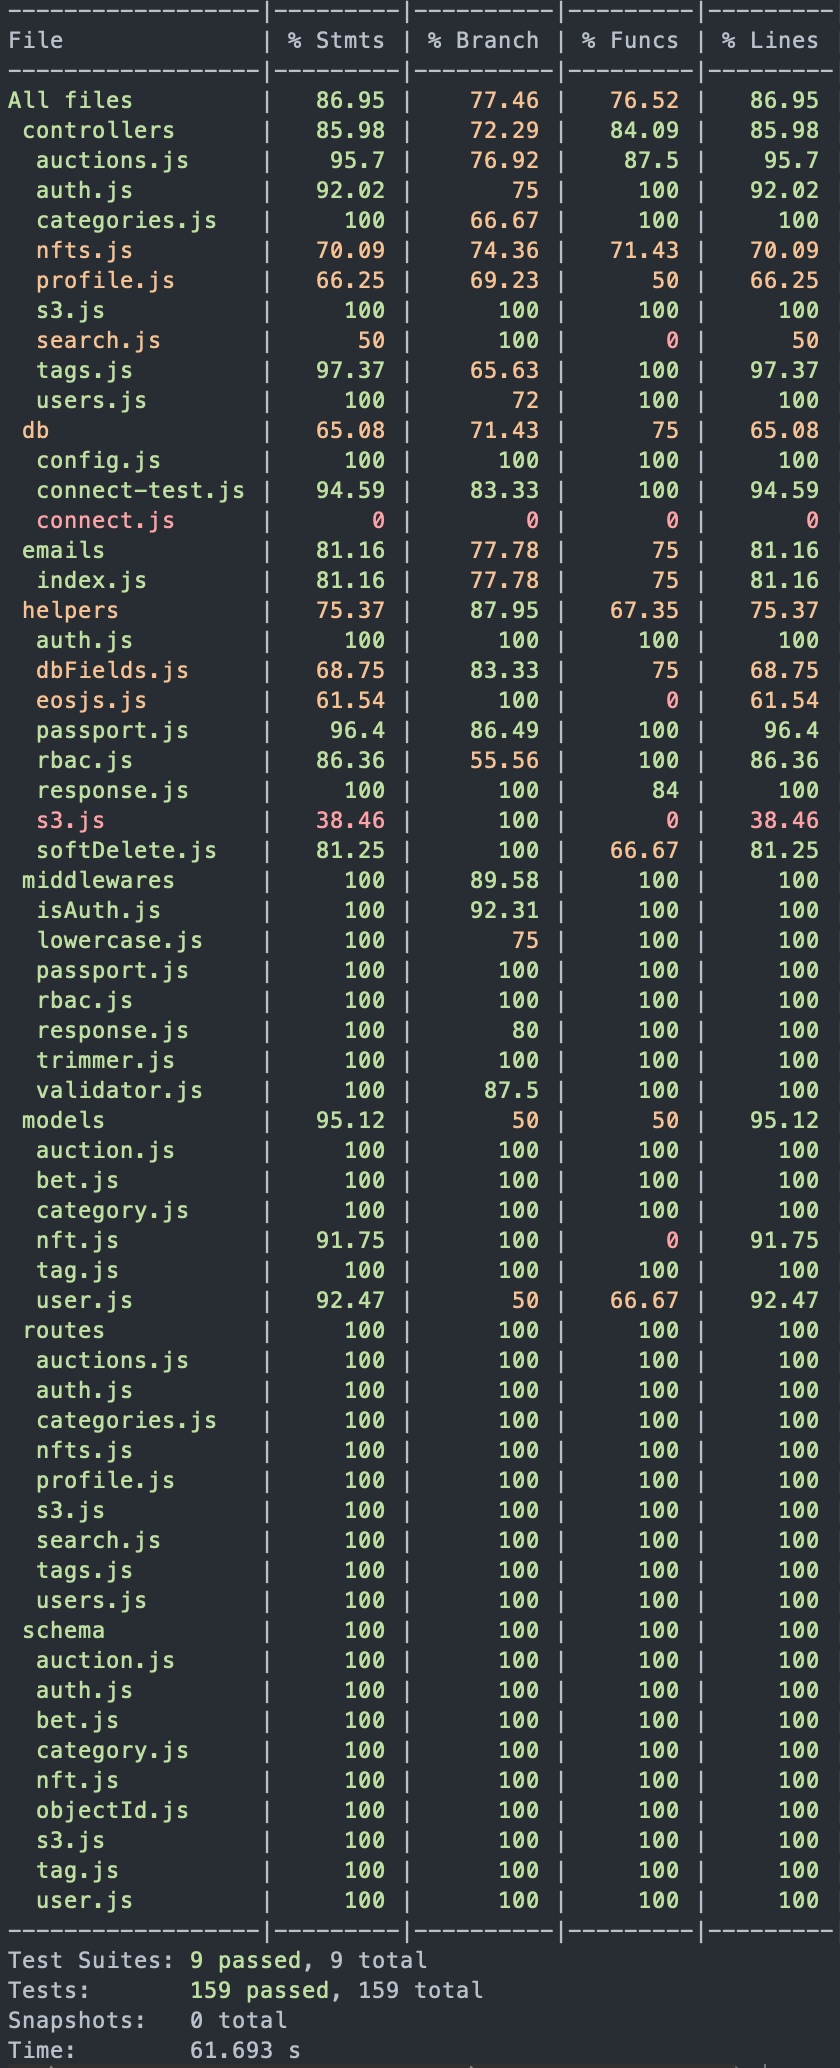
\includegraphics[width=0.40\textwidth,keepaspectratio]{api-test.jpg}
	\caption{Test coverage della RestApi}
	\label{fig:apiTest}
\end{figure}

\begin{figure}[H]
	\centering
	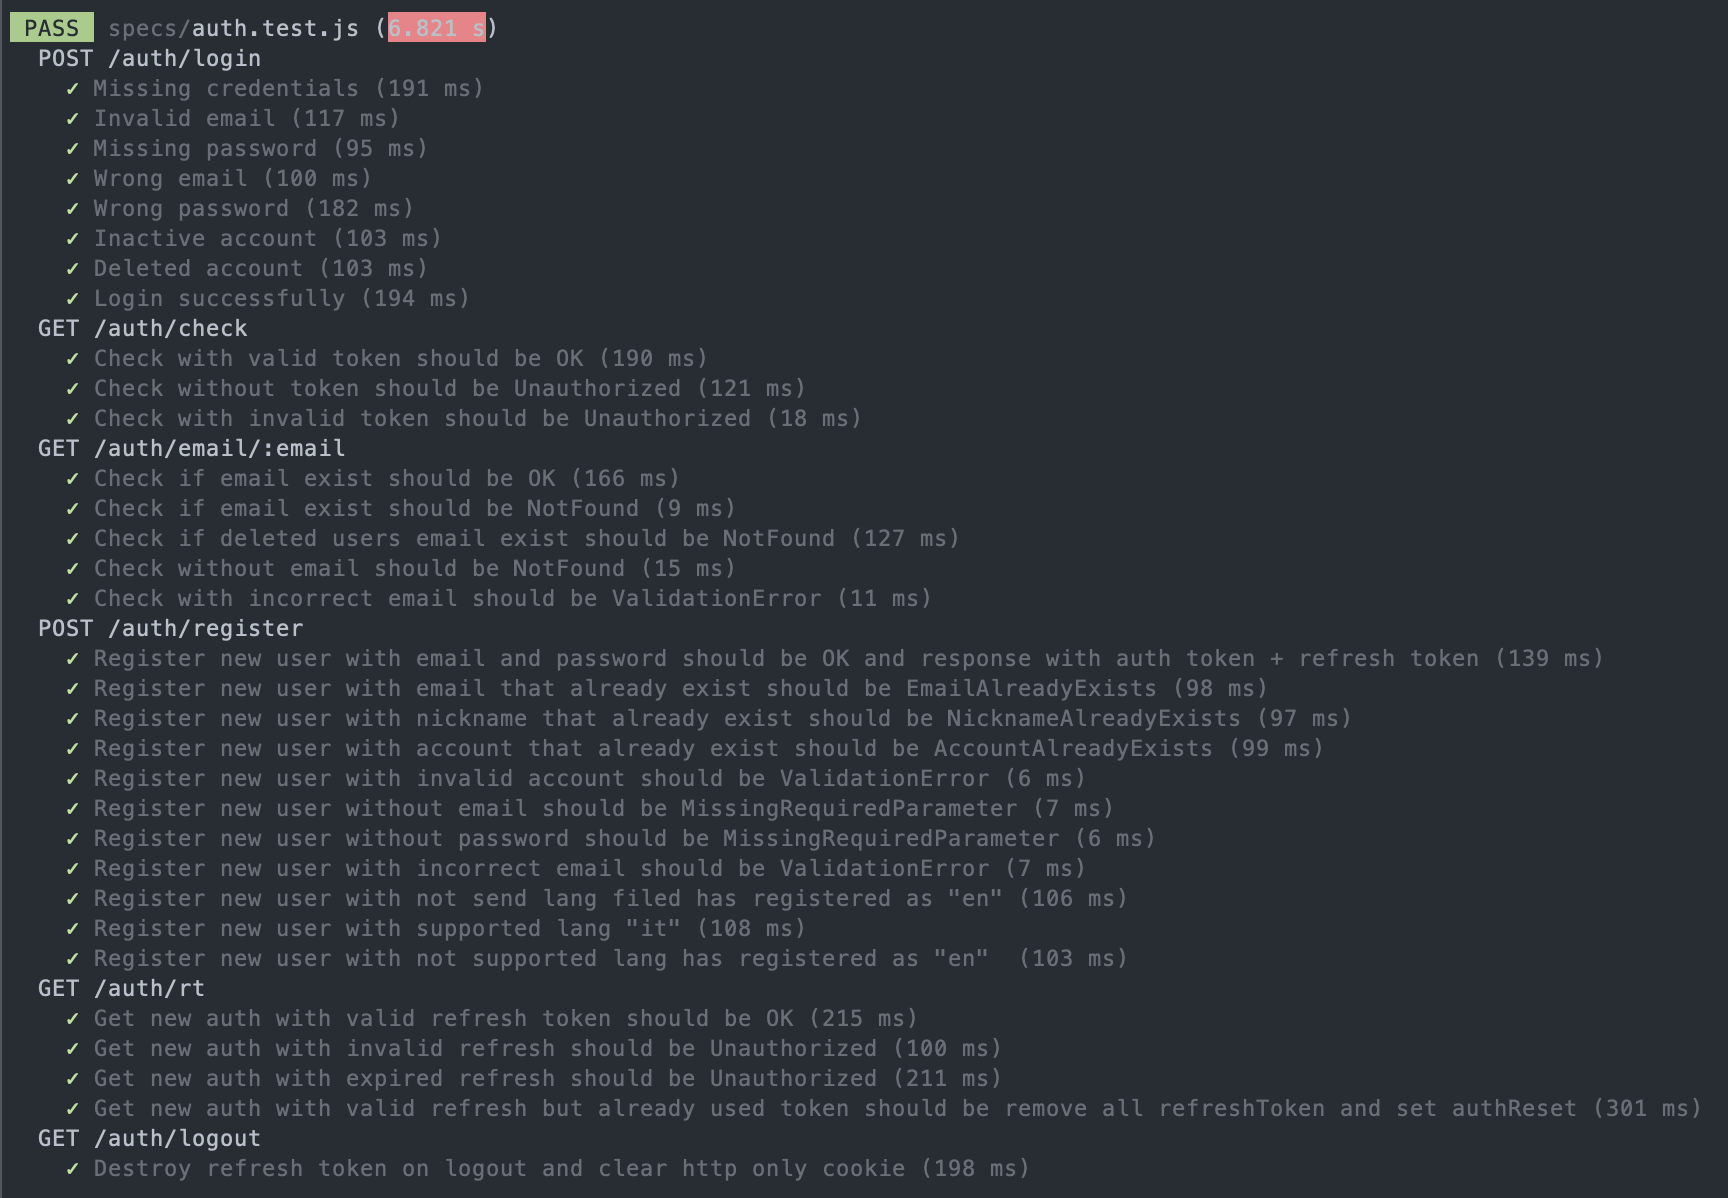
\includegraphics[width=\textwidth,keepaspectratio]{auth-test.jpg}
	\caption{Test dell'endpoint /auth per l'autenticazione}
	\label{fig:authTest}
\end{figure}

\begin{figure}[H]
	\centering
	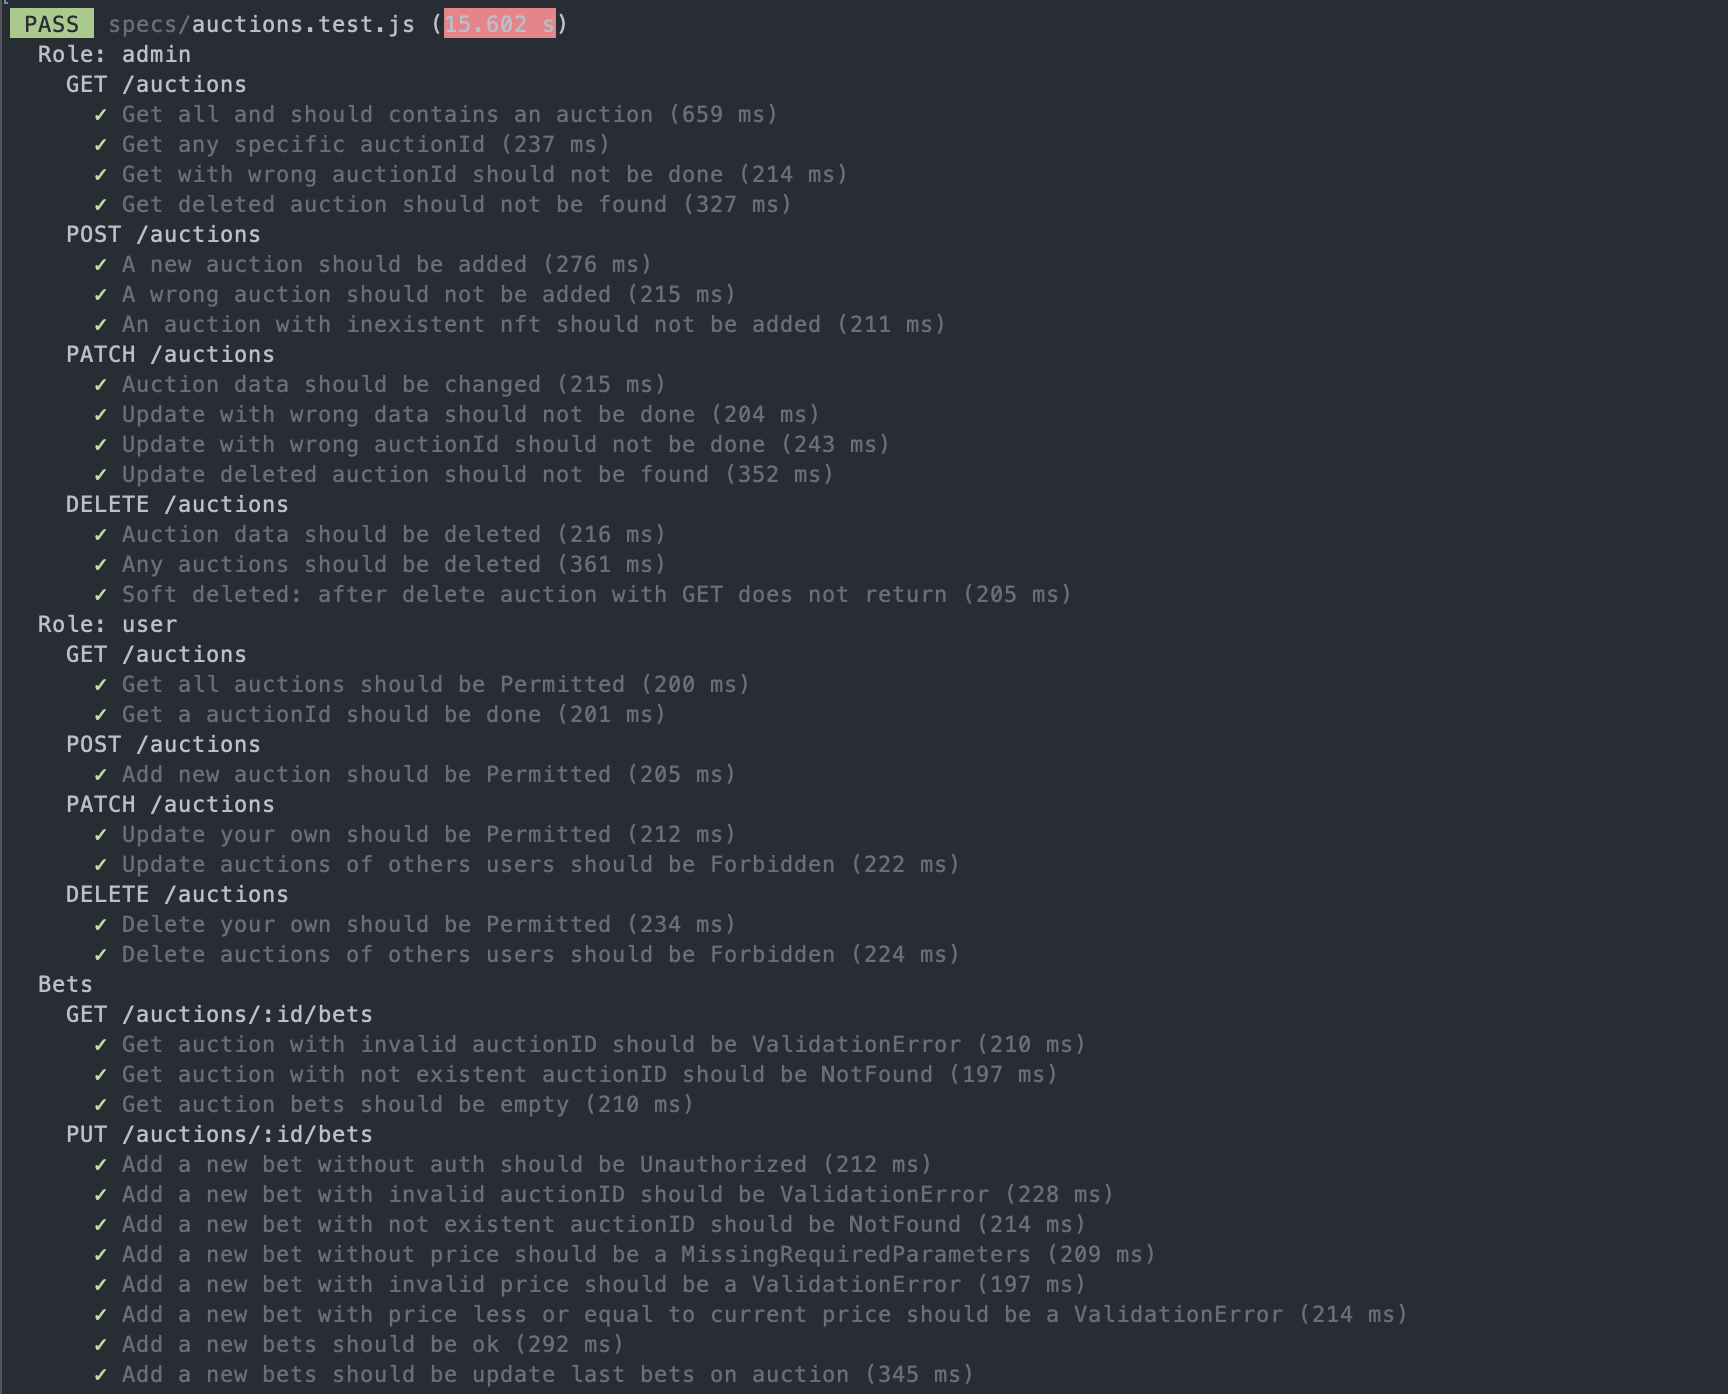
\includegraphics[width=\textwidth,keepaspectratio]{auctions-test.jpg}
	\caption{Test dell'endpoint /auctions delle aste}
	\label{fig:auctionsTest}
\end{figure}

\clearpage

\subsection{User Experience}
Verso le fasi finali del progetto, quando avevamo ormai un prototipo funzionante, abbiamo deciso di mostrarlo ad alcune persone, per l'esattezza 3, per raccogliere feedback sulla UserExperience.
Tra queste persone c'era anche l'ideatore del progetto, una persona esterna al team ma che ci aveva lanciato l'idea in quanto sua esigenza e vorrebbe investire in un portale di questo tipo.

Principalmente, sono emersi due problemi:

\begin{itemize}
	\item Mancanza di feedback concreti una volta che l'utente effettuava la puntanta, non era sicuro che fosse andata a buon fine.
	\item Grazie al socket, quando un utente sta guardando la pagina dell'asta, 
	nel caso in cui arrivasero nuove offerte viene aggiunto un nuovo elemento nella lista delle puntate.
	Anche in questo caso, la mancanza di feedback visivi, non permetteva agli utilizzatori di notarlo rapidamente.
	\item Necessità di sapere che l'attuale offerta pià alta sia della persona collegata al portale.
\end{itemize}
\bigbreak
\noindent
Grazie a questi feedback, abbiamo migliorata la User Interface come segue.
\clearpage

\begin{figure}[H]
	\centering
	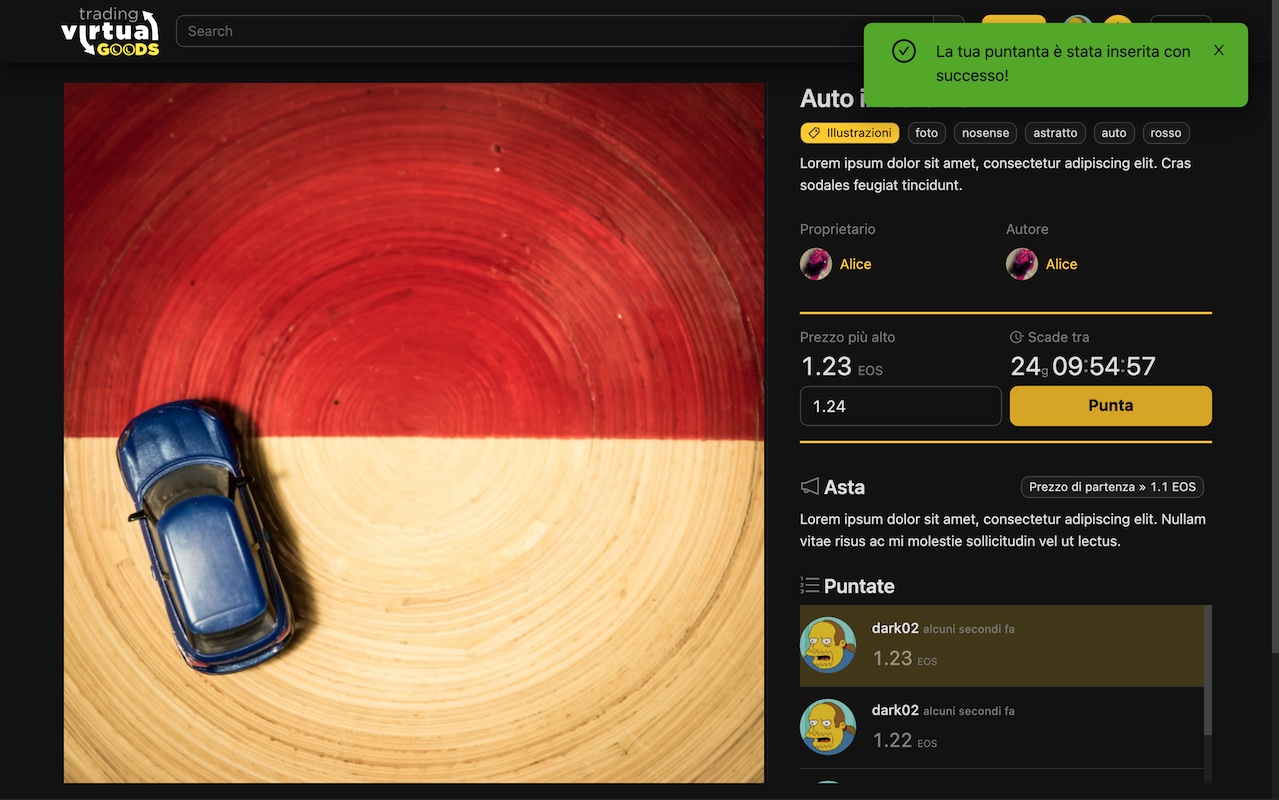
\includegraphics[width=0.80\textwidth,keepaspectratio]{test-feedback-desktop.jpg}
	\caption{Feedback desktop dopo una puntata}
	\label{fig:testFeedbackDesktop}
\end{figure}
\begin{figure}[H]
	\centering
	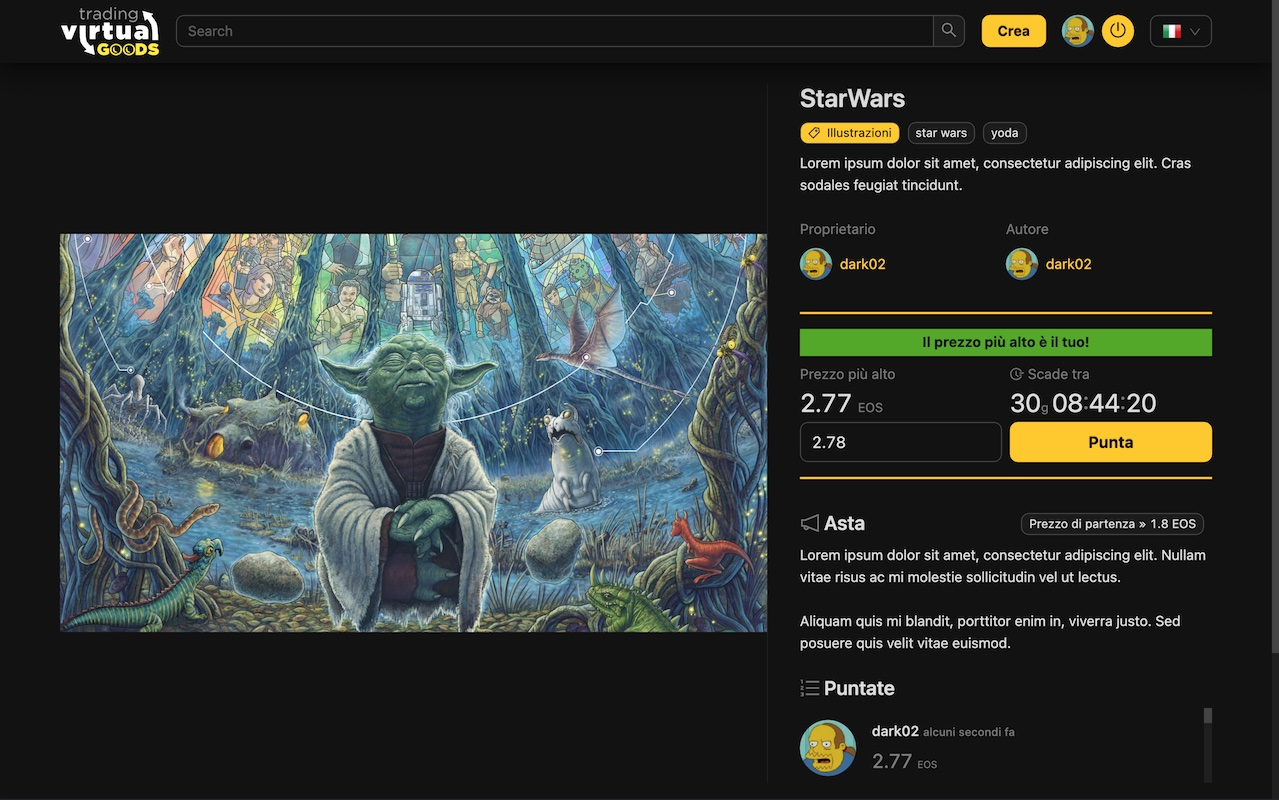
\includegraphics[width=0.80\textwidth,keepaspectratio]{test-hightest-desktop.jpg}
	\caption{Visualizzazione desktop offerta più alta}
	\label{fig:testHightestDesktop}
\end{figure}

\begin{figure}[H]
	\centering
	\begin{minipage}[b]{0.48\textwidth}
		\centering
		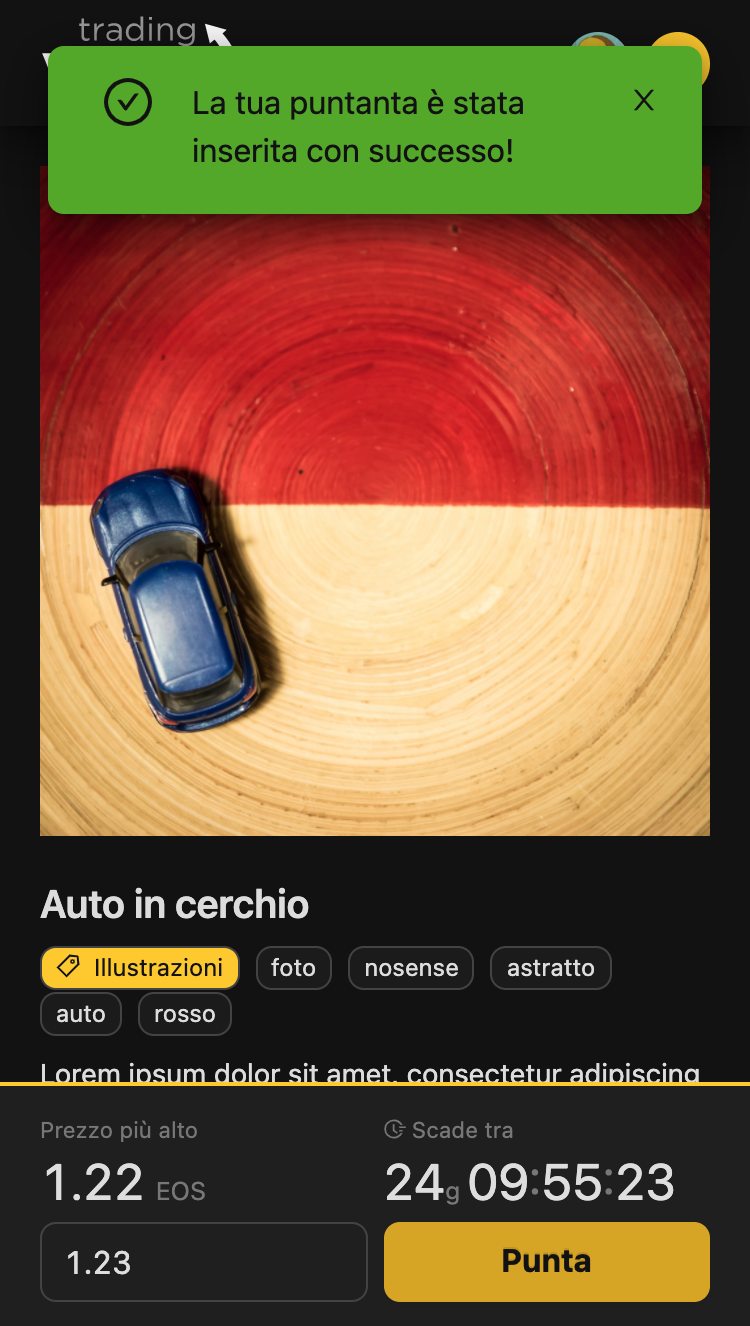
\includegraphics[width=\linewidth,keepaspectratio]{test-feedback-mobile.jpg}
		\caption{Feedback mobile\\dopo una puntata}
		\label{fig:testFeedbackMobile}
	\end{minipage}
	\begin{minipage}[b]{0.48\textwidth}
		\centering
		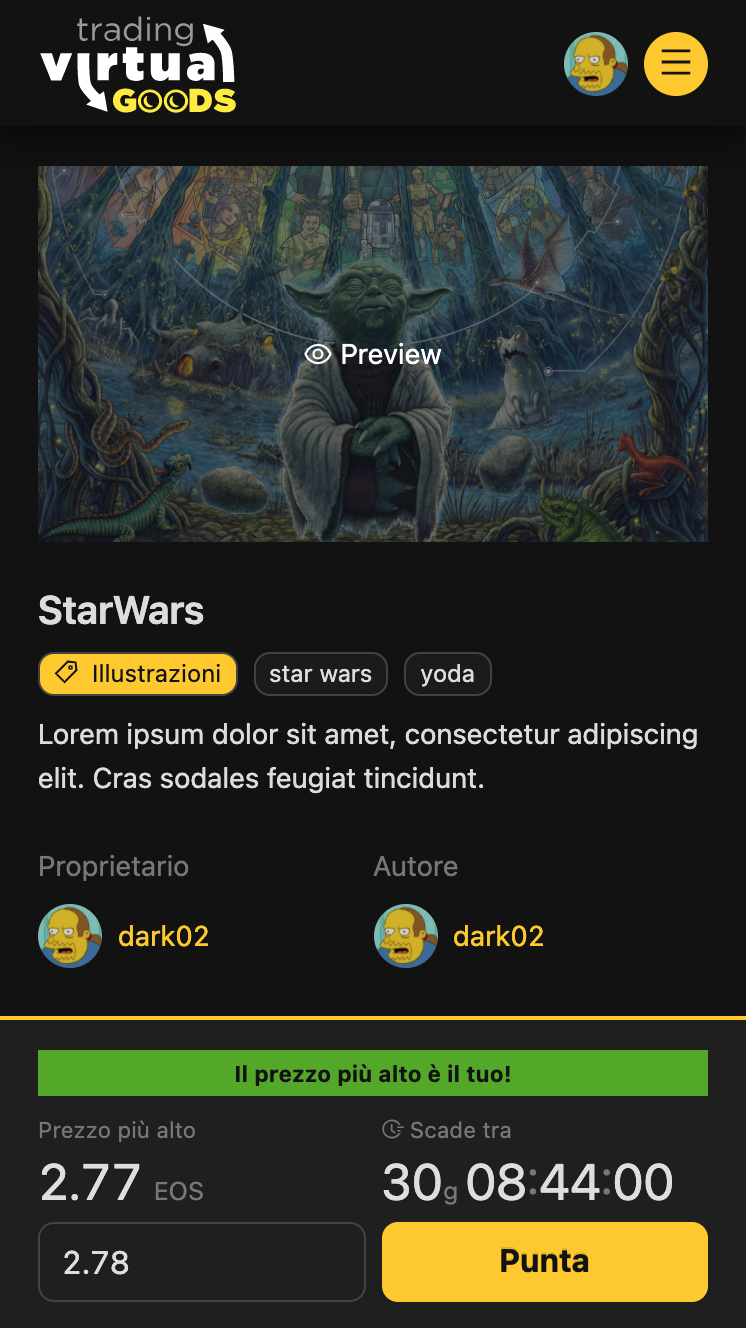
\includegraphics[width=\linewidth,keepaspectratio]{test-hightest-mobile.jpg}
		\caption{Visualizzazione desktop\\offerta più alta}
	\label{fig:testHightestMobile}
	\end{minipage}	
\end{figure}